\documentclass[aspectratio=169, 8pt, xcolor={svgnames}]{beamer}
\usetheme[progressbar=frametitle]{metropolis}
\setbeamercolor{background canvas}{bg=white}
\setbeamerfont{footnote}{size=\tiny}
\usepackage{hyperref}

% Impostazioni per il colore dei link
\hypersetup{
    colorlinks=true,    % Attiva i colori per i link
    linkcolor=black, % Colore dei link interni
    urlcolor=persianred        % Colore dei link esterni (url)
}
\usepackage{appendixnumberbeamer}
\usepackage{url}
\usepackage{amsfonts} 
\usepackage{amssymb}
\usepackage[english]{babel}
\usepackage{fontawesome}
\usepackage{multicol}
\usepackage{braket}
\usepackage{overpic} 
\usepackage{bm}
\usepackage{braket}
\usepackage{algorithm}
\usepackage{algpseudocode}
\usepackage{enumitem}

\usepackage[]{pseudo}

\usepackage{tikz}
\usetikzlibrary{positioning,arrows,calc,math,angles,quotes}
\usepackage{blochsphere}

\newcommand{\quotes}[1]{``#1''}

\DeclareMathAlphabet{\mathpzc}{OT1}{pzc}{m}{it}

\renewcommand\L{\hat L}
\newcommand{\qu}{\hat Q}
\newcommand{\X}{\hat X}
\newcommand{\Y}{\hat Y}
\newcommand{\Z}{\hat Z}
\newcommand{\XXZ}{\operatorname{XXZ}}
\renewcommand\d[1]{\Delta(#1)}
\renewcommand\o[1]{\sigma(#1)}
\newcommand\etak[1]{\eta^{\mtiny{(#1)}}}
\def\w{\hat W}
\def\h{\hat H}
\def\D{\hat D}
\def\v{\hat V}
\def\bfzero{\boldsymbol{0}}
\def\bftheta{\boldsymbol{\theta}}
\def\vqe{\u_{\bftheta}}
\def\vqes{\u_{\bftheta}}

\newcommand{\sandwich}[3]
  {\left\langle  #1 \right| #2 \left| #3 \right\rangle}


\def\U{\hat{ \mathcal U}}
\def\H{{\hat{ \mathcal H}}}
\def\W{\hat{ \mathcal W}}
\def\dell{{\delta\ell}}
\def\dell{{\mathpzc {S}}}
\def\dell{{s}}
\def\S{\mathbf{s}}
\def\delll{{\delta w}}
\def\dells{{u}}
\def\delll{{\mathpzc R}}
\def\delll{{w}}
\def\p{\Z}
\def\hell{{\h_\ell}}
\def\Hell{{{\H}_\ell}}
\def\well{{\w_\ell}}
\def\Well{{\W_\ell}}
\def\ohell{\o{\h_\ell}}
\def\oHell{\o{\H_\ell}}
\def\dhell{\d{\h_\ell}}
\def\dHell{\d{\H_\ell}}
\def\Ell{\overline{\ell}}
\def\Uell{{\U_\ell}}
\def\u{{\hat U}}
\def\uell{{\u_\ell}}
\def\Q{\hat Q}
\def\D{\hat D}
\def\Dbf{\mathbf{\hat D}}
\def\Upsi{U^{(\psi)}}
\newcommand{\Upsik}[1]{U^{(\psi_{#1})}}
\newcommand{\Vpsik}[1]{V^{(\psi_{#1})}}

\def\vDBI{\hat R}
\def\VDBI{\mathcal T}
\def\UDBI{\mathcal V}
\def\RDBI{\hat R}
\def\PDBI{\mathcal P}

\def\I{\mathcal I}
\def\delln{{\dell^{\mtiny{(N)}}}}
\def\elln{\ell^{\mtiny{(N)}}}
\def\wn{\w^{\mtiny{(N)}}}
\def\wnm{\w^{\mtiny{(N-1)}}}
\def\un{\u^{\mtiny{(N)}}}
\def\unm{\u^{\mtiny{(N-1)}}}
\def\hn{{\h^{\mtiny{(N)}}}}
\def\hnm{{\h^{\mtiny{(N-1)}}}}
\def\wtn{\w^{\mtiny{\rceil N\rfloor}}}
\def\utn{\w^{\mtiny{\rceil N\rfloor}}}
\def\htn{\w^{\mtiny{\rceil N\rfloor}}}
\def\dellnm{\dell^{\mtiny{(N-1)}}}
\def\D{\mathcal D}
\def\Z{\hat Z}
\def\Pr{\mathrm{Pr}}
\newcommand\sntc[2]{\Delta^{#1}(#2)}
\def\snt{\sntc n\ell}
\def\snr{\sntc n r}
\def\snst{}
\def\dtn {\mathrm{d}^ns}
\def\dr {\mathrm{d} r}
\newcommand\dtnc[2]{\mathrm{d}^{#1}#2}
\def\dd {\mathrm{d}}
\def\bc{\{0,1\}^{\times L}}
\def\zm{\Z_\mu}
\newcommand\zmc[1]{\Z_{\etak {#1}}}
\def\xn{\X_\nu}
\def\zmp{\Z_{\mu^{\prime}}}
\def\xnp{\X_{\nu^{\prime}}}
\def\mnbc{{\mu,\nu \in \bc}}
\def\mbc{{\mu \in \bc}}
\def\hmn{\overline {H}_{\mu,\nu}}
\def\RBS{\operatorname{RBS}}

\def\A{\hat A}
\def\B{\hat J}
\def\drr{r^{\prime}}
\def\linops{{\mathcal L(\CC^{\times D})}}
\def\A{\hat A}
\def\B{\hat B}
\def\C{\hat C}
\def\D{\hat D}
\def\NC{\mathcal N}
\def\n{K}
\def\elk{\ell_k}
\def\elkm{{{\ell_{k-1}}}}
\def\rxi{\mathcal R_k(s)}
\def\phk{\partial \h_{k-1}}
\def\G{\mathcal{N}_W(K)}
\def\vgc{\v^{\mtiny{\mathrm{(GC)}}}}
\def\vmp{\v^{\mtiny{\mathrm{(\mu_1,\ldots,\mu_R)}}}}
\def\vd{\v^{\mtiny{(\Delta)}}}
\def\elk{\ell_k}
\def\elkm{\ell_{k-1}}
\def\wz{{\w^{\mtiny{(Z)}}}}
\def\wmu{{\w^{\mtiny{(\mu)}}}}
\def\dzz{\Delta^{\mtiny{(Z)}}}
\def\dmu{\overline{\Delta^{\mtiny{(\eta)}}}}
\def\vk{\v_k}
\def\vkm{\v_{k-1}}
\def\b{B}
\def\bk{\b_k}
\def\J{\hat A}
\def\Jk{\J_k}
\def\Jkm{\J_{k-1}}
\def\sgd{$\sigma$-decreasing }
\def\pch{\hat Q}

\usetikzlibrary{arrows,automata}
\usetikzlibrary{positioning}
\usetikzlibrary{arrows.meta,
                bending,
                intersections,
                quotes,
                shapes.geometric}

\tikzset{
    state/.style={
           rectangle,
           rounded corners,
           draw=black, very thick,
           minimum height=1em,
           inner sep=2pt,
           text centered,
           },
}

\definecolor{myv}{rgb}{0.36, 0.22, 0.33}
\definecolor{gio}{rgb}{0.45, 0.31, 0.59}
\definecolor{light}{rgb}{0.8, 0.8, 1}
\definecolor{warmblack}{rgb}{0.0, 0.26, 0.26}
\definecolor{brown(web)}{rgb}{0.65, 0.16, 0.16}
\definecolor{cadmiumgreen}{rgb}{0.0, 0.42, 0.24}
\definecolor{darkmidnightblue}{rgb}{0.0, 0.2, 0.4}
\definecolor{brightube}{rgb}{0.82, 0.62, 0.91}
\definecolor{bleudefrance}{rgb}{0.19, 0.55, 0.91}
\definecolor{brightmaroon}{rgb}{0.76, 0.13, 0.28}
\definecolor{codegreen}{rgb}{0,0.6,0}
\definecolor{codegray}{rgb}{0.5,0.5,0.5}
\definecolor{codepurple}{rgb}{0.58,0,0.82}
\definecolor{backcolour}{rgb}{0.95,0.95,0.92}
\definecolor{amethyst}{rgb}{0.6, 0.33, 0.73}
\definecolor{mediumpersianblue}{rgb}{0.0, 0.4, 0.65}
\definecolor{persianred}{rgb}{0.8, 0.2, 0.2}
\definecolor{deepcarrotorange}{rgb}{0.91, 0.41, 0.17}

\usepackage[most]{tcolorbox}
\usepackage{xcolor}


\title{Boosting ground states preparation with double-bracket quantum algorithms}
\subtitle{\texttt{PART 1:} Introducing and optimizing double-bracket quantum algorithms}
\date{28 November 2024}
\author{Matteo Robbiati}
\titlegraphic{
   \begin{tikzpicture}[overlay, remember picture]
   \node[at=(current page.south east), anchor=south east] {%
      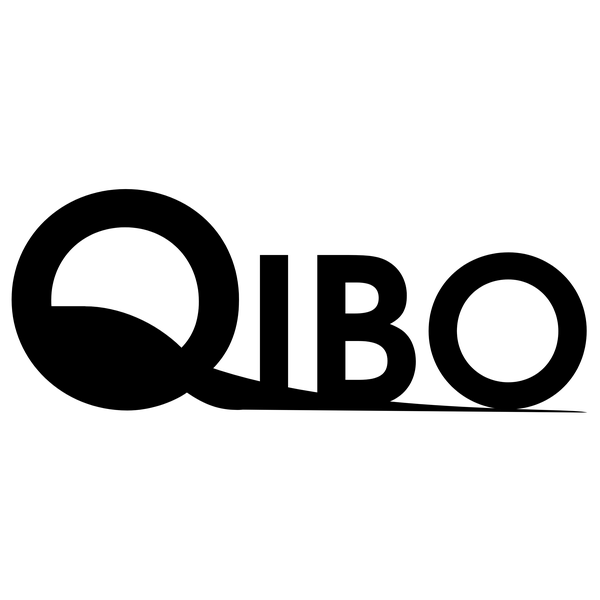
\includegraphics[width=.15\textwidth]{figures/qibo.png} 
      
\includegraphics[width=.15\textwidth]{figures/unimi.png} 
      
\includegraphics[width=.15\textwidth]{figures/cern.png}  
      
\includegraphics[width=.15\textwidth]{figures/qti.png}  
   };
   \end{tikzpicture}
}

\begin{document}

\begin{frame}
\maketitle
\end{frame}

\begin{frame}{A couple of references}
\begin{multicols}{2}
\begin{figure}
   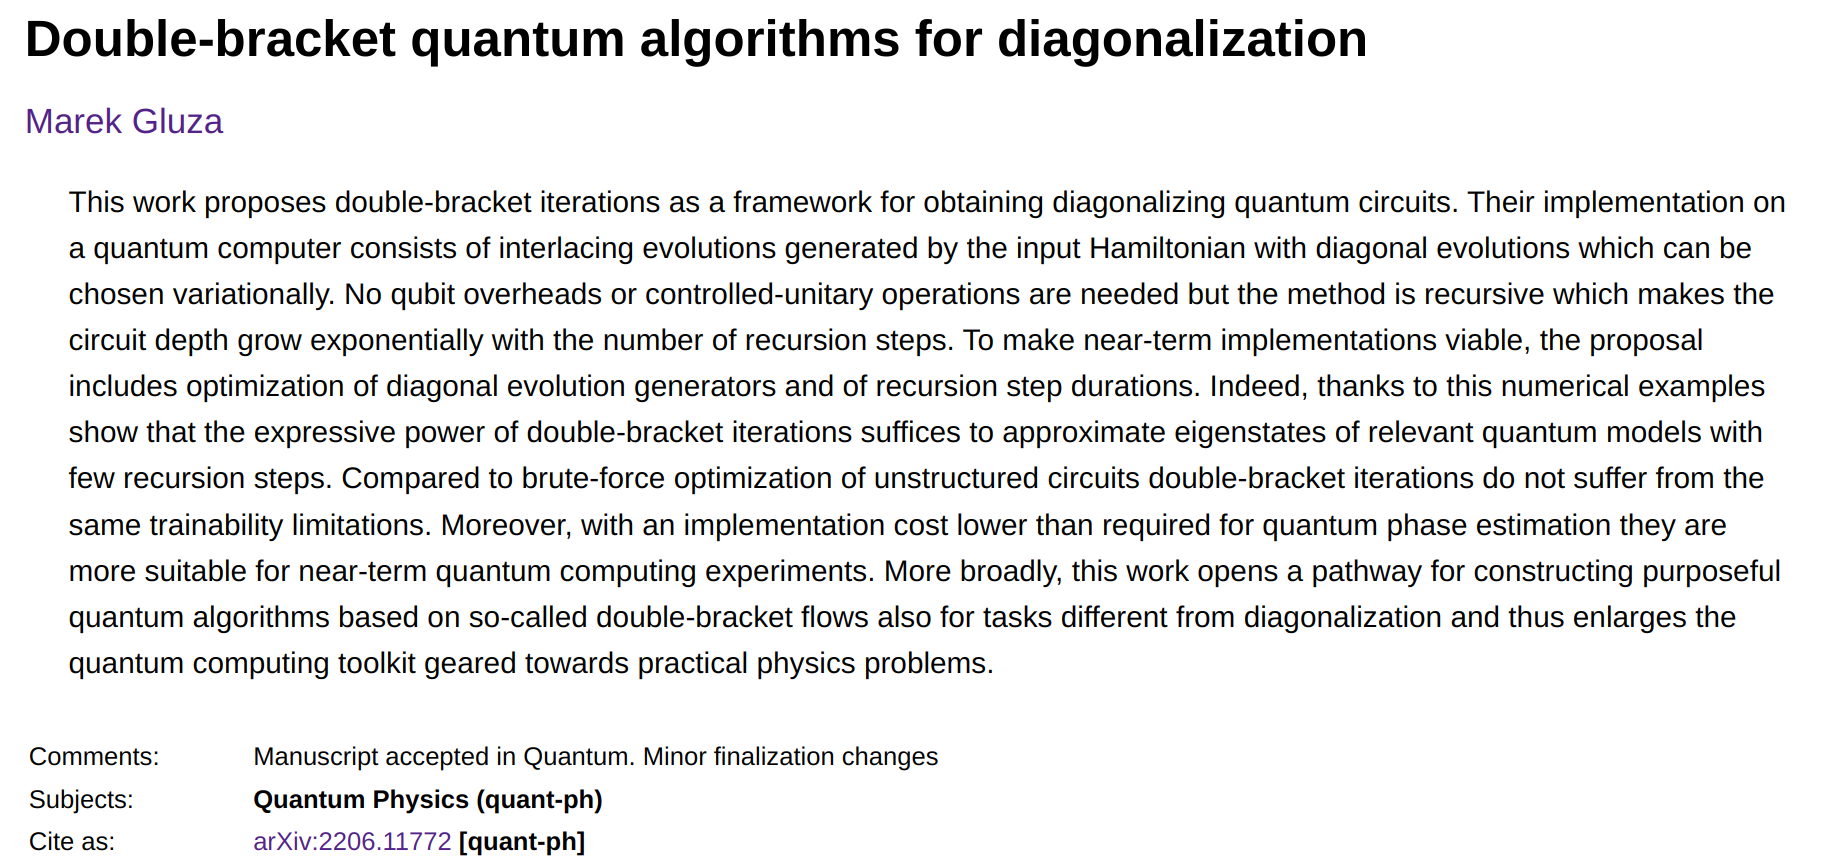
\includegraphics[width=0.5\textwidth]{figures/dbqa_paper.png}
\end{figure}
Check out this because:
\begin{itemize}[noitemsep]
\item[1.] Marek is a very nice and smart guy;
\item[2.] it contains math foundations of this talk; 
\end{itemize}
\begin{figure}
   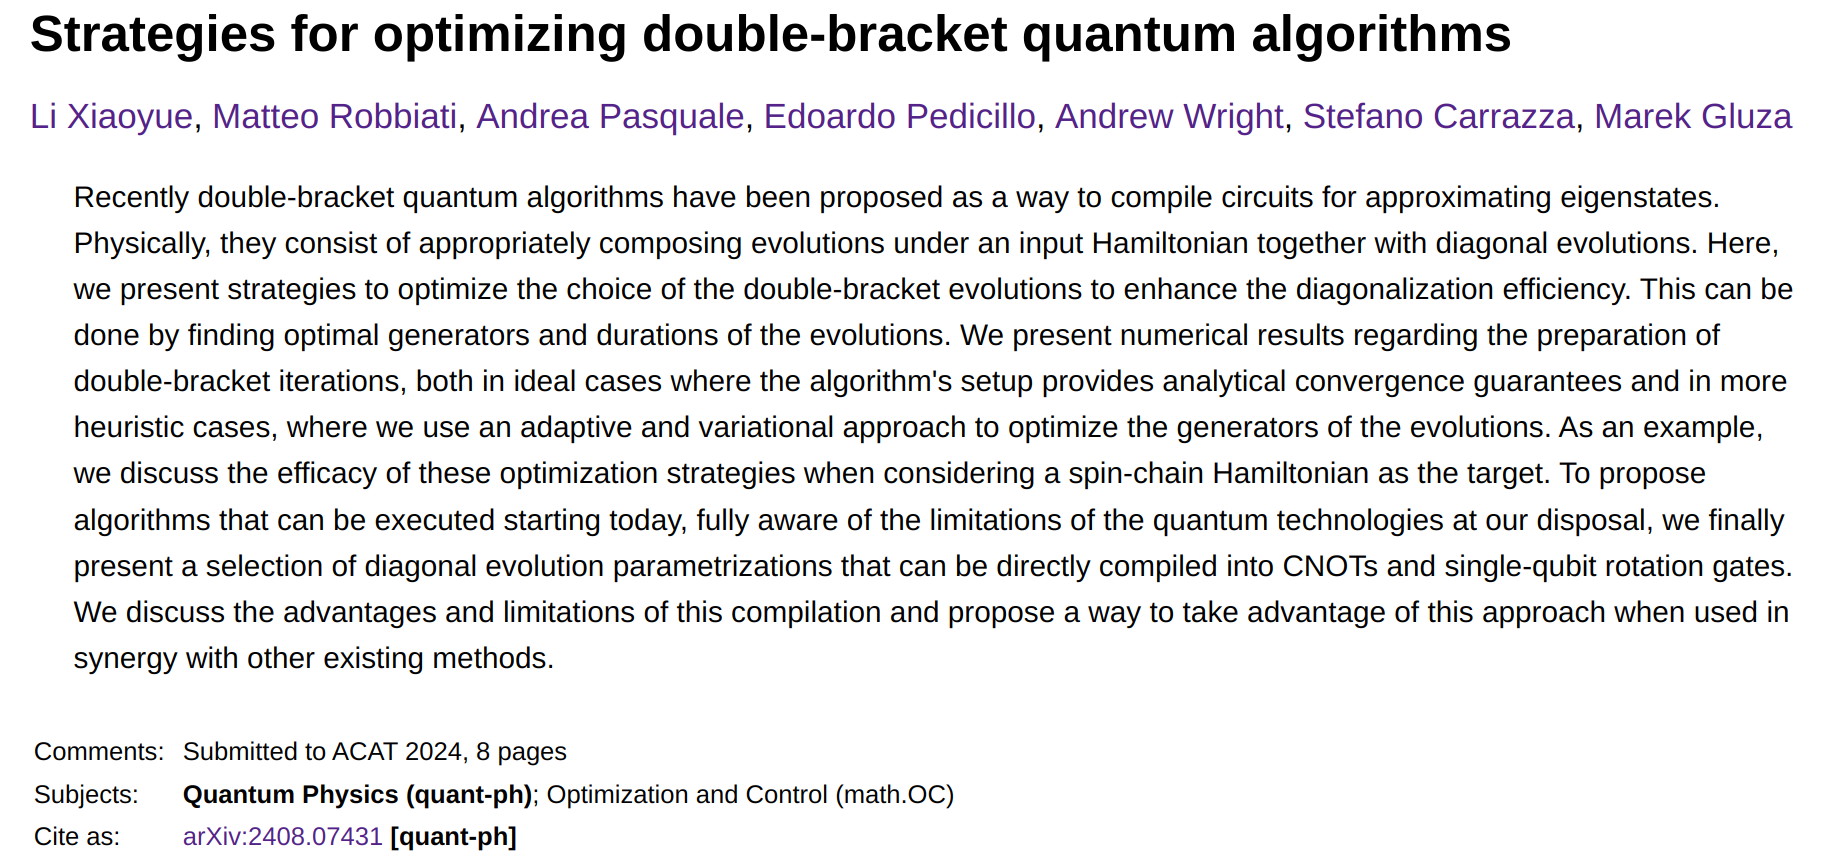
\includegraphics[width=0.5\textwidth]{figures/dbqa_opt.png}
\end{figure}
And this because:
\begin{itemize}[noitemsep]
\item[1.] We delve deeper into the optimization of DBQAs;
\item[2.] we base the optimization of the next talk on these studies. 
\end{itemize}
\end{multicols}
\end{frame}

\begin{frame}{Double-bracket iterations \hfill \href{https://arxiv.org/abs/2206.11772}{\textcolor{white}{\faBook\,\,arXiv:2206.11772}}}
\begin{columns}[T,onlytextwidth]
    % First column: 40%
    \begin{column}{0.45\textwidth}
    \textbf{Ingredients}
        \begin{itemize}[noitemsep]
            \item[1.] Input Hamiltonian $\textcolor{mediumpersianblue}{\hat H_0}$ (here 1D XXZ);
            \item[2.] an anti-hermitian ($(i\hat{W})^{\dagger} = -i\hat{W}$) rotation generator $\textcolor{persianred}{\hat{W}_0} = [\hat{D}_0, \hat H_0]$;
            \item[3.] point 2. is used to build a unitary operation:
              $$ \hat{R}_0 \equiv e^{s \textcolor{persianred}{\hat{W}_0}}, $$
              with $s$ stepsize or flow duration;
            \item[4.] $\hat{R}_0$ applied to $\hat{H}_0$ as \textit{double-bracket rotation}:
               $$ \hat H_1 =  e^{s\textcolor{persianred}{\hat{W}_0}} \textcolor{mediumpersianblue}{\hat H_0} e^{- s \textcolor{persianred}{\hat{W}_0}}.$$
        \end{itemize}

    \end{column}

    % Second column: 60%
    \begin{column}{0.55\textwidth}
        \begin{figure}
           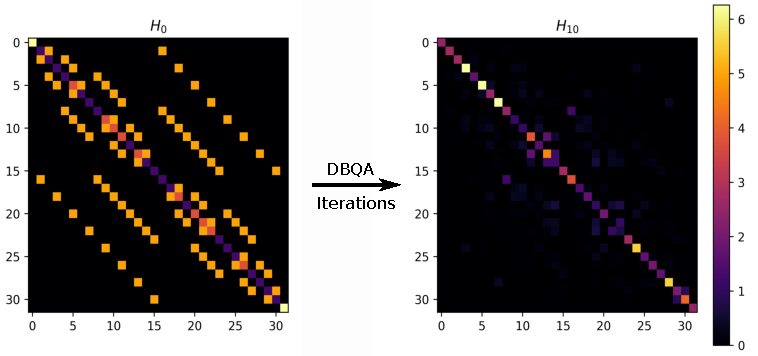
\includegraphics[width=0.95\textwidth]{figures/dbqa_10steps.pdf}
        \caption{Ten DBQA rotations to a 5 qubit 1D XXZ.}
        \end{figure}
    \end{column}
\end{columns}
\begin{tcolorbox}[colback=red!15, title=Nomenclature reason]
The presented framework satisfies a Heisenberg equation involving two, not one, brackets:
$$ \partial_s \hat{H}_0(s) = [ \hat{H}_0(s), [ \hat{H}_0(0), \hat{D}_0 ] ]. $$
\end{tcolorbox}
\end{frame}

\begin{frame}{Some properties and important notes \hfill \href{https://arxiv.org/abs/2206.11772}{\textcolor{white}{\faBook\,\,arXiv:2206.11772}}}
\begin{itemize}[noitemsep]
\item[1.] We care of diagonal 
   $\hat{D}_k$ in $\hat{W}_k = [\hat{D}_k, \hat{H}_k]$. A natural choice is the canonical
   generator\footnote{See \href{https://journals.aps.org/prd/abstract/10.1103/PhysRevD.48.5863}{Renormalization of Hamiltonians, Glazek and Wilson, 1993} and 
   \href{https://onlinelibrary.wiley.com/doi/abs/10.1002/andp.19945060203}{Flow-equations for Hamiltonians, Wegner, 1994} for extras.}:
   $$ 
   \hat{W}_k^{\rm can} = [\hat{H}_k, \hat{\Delta}(\hat{H}_k)], \qquad \text{with} \qquad  
   \begin{cases}
   \hat{\Delta}(\hat{H}_k) = \text{diag}(\hat{H}_k), \\
   \hat{H}_k = \hat{\Delta}(\hat{H}_k) + \hat{\sigma}(\hat{H}_k),
   \end{cases}
   $$
   but - as we will see - many choices can be done here.
\item[2.] \textbf{Lemma}\footnote{Definition and proof of Lemma 2 in \href{https://arxiv.org/abs/2206.11772}{Double-bracket 
   quantum algorithms for diagonalization, M. Gluza, 2024}}: given $\sigma(\hat{H}_0(s))$ off-diagonal restriction of $\hat{H}_0(s)$ and
   $s$ small enough:
   $$ \partial_s \| \sigma(\hat{H}_0(s)) \|^2_{\rm HS} = - 2 \braket{ \hat{W}_0, 
   [\hat{H}_0, \sigma(\hat{H}_0(s))] }_{\rm HS}. $$ 
\item[3.] If $\hat{D}_0 = ... = \hat{D}^*$, as long as $s_0 = ... = s^*$
   are sufficiently small and $\hat{D}^*$ non degenerate, the recursion converges to a fixed point $\hat{H}_{\infty}$
   with $[\hat{H}_{\infty}, \hat{D}^*]$\footnote{\textbf{If you are really brave:} 
   \href{https://link.springer.com/book/10.1007/978-1-4471-3467-1}{Optimization and Dynamical Systems [Ch. 2.3], Uwe Helmke , John B. Moore, 1994.}}; 
\end{itemize}
\begin{tcolorbox}[colback=red!15]
\begin{itemize}[noitemsep]
\item[$2. \to$] If $\hat{D}_0$ is diagonal, then $\hat{H}_1$ will be more diagonal than $\hat{H}_0$,
\item[$3. \to$] the discrete DBI can converge arbitrary well,
\item[$3. \to$] \textit{analytically motivated} methods work in some setups but they can be slow.
\end{itemize}
\end{tcolorbox}
\begin{picture}(0,0)
    \put(325,30){
        
\includegraphics[width=0.12\textwidth]{figures/take_away.png}
    }
\end{picture}
\end{frame}

\begin{frame}{Cost functions and parametrization strategies \hfill \href{https://arxiv.org/abs/2408.07431}{\textcolor{white}{\faBook\,\,arXiv:2408.07431}}}
\begin{figure}
   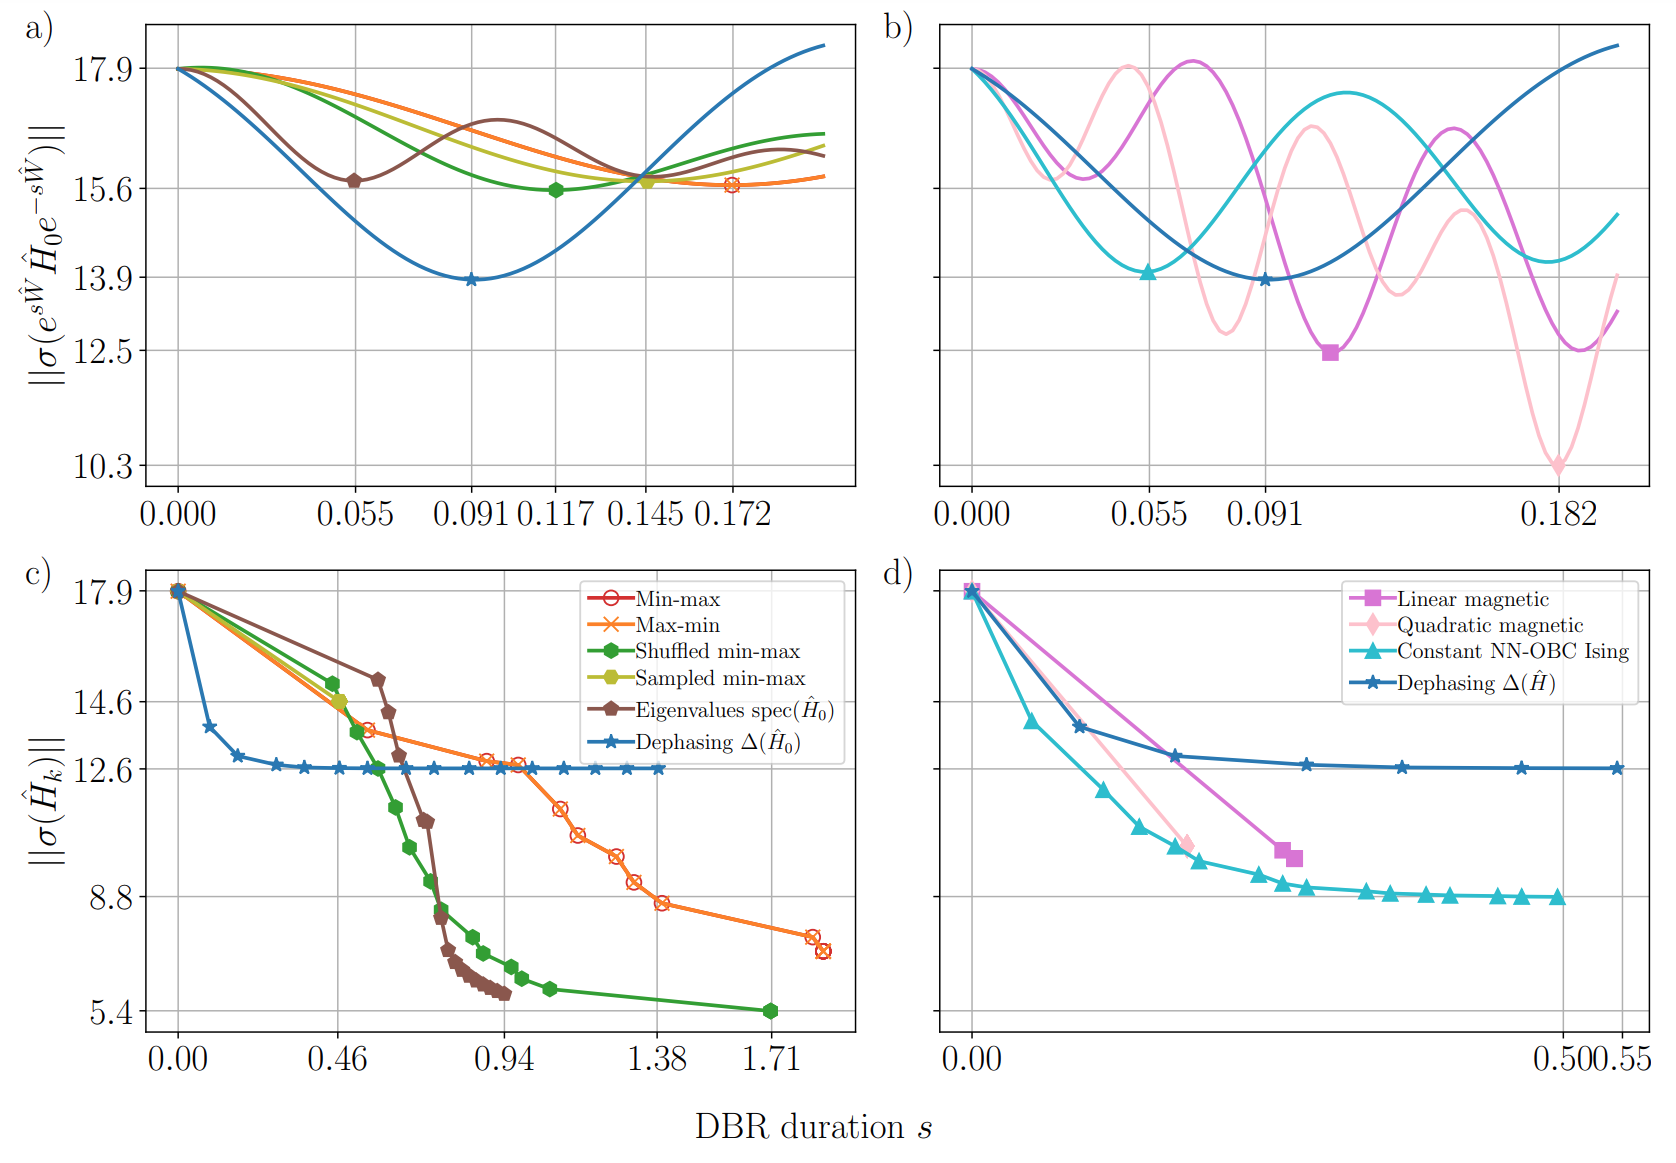
\includegraphics[width=0.6\textwidth]{figures/opt_strategies.png}
\end{figure}
\vspace{-0.2cm}
\begin{figure}
   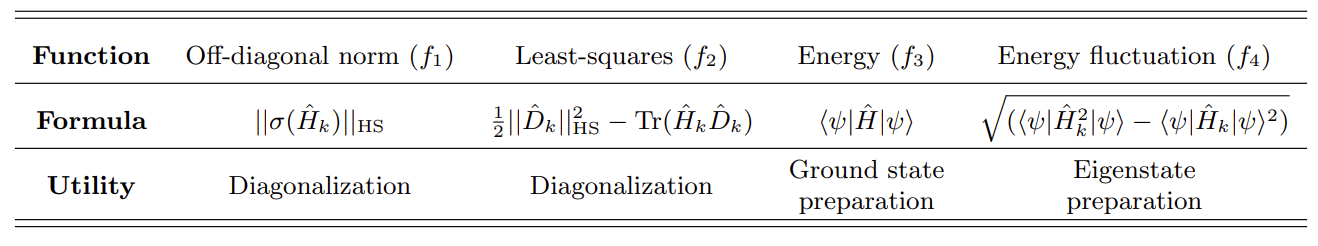
\includegraphics[width=0.7\textwidth]{figures/cost_functions.png}
\end{figure}
\begin{picture}(0,0)
    \put(335,150){
        
\includegraphics[width=0.15\textwidth]{figures/variational_icon.pdf}
    }
\end{picture}
\begin{picture}(0,0)
    \put(0,150){
        
\includegraphics[width=0.15\textwidth]{figures/analytical_icon.pdf}
    }
\end{picture}
\begin{picture}(0,0)
    \put(-20,40){
        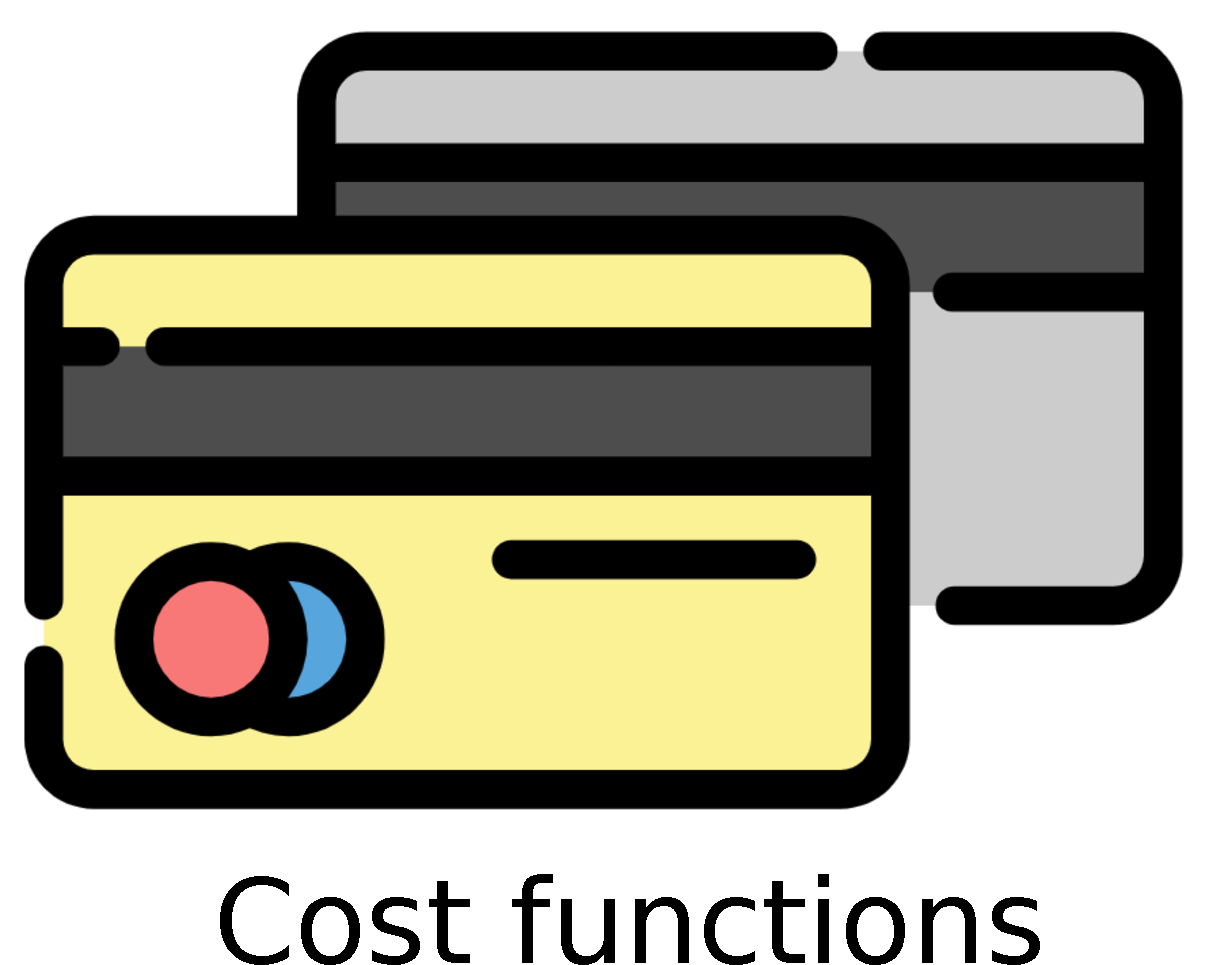
\includegraphics[width=0.15\textwidth]{figures/cost_icon.pdf}
    }
\end{picture}
\end{frame}

\begin{frame}{Double-bracket rotations can be optimized \hfill \href{https://arxiv.org/abs/2408.07431}{\textcolor{white}{\faBook\,\,arXiv:2408.07431}}}
\begin{center}
\begin{figure}
   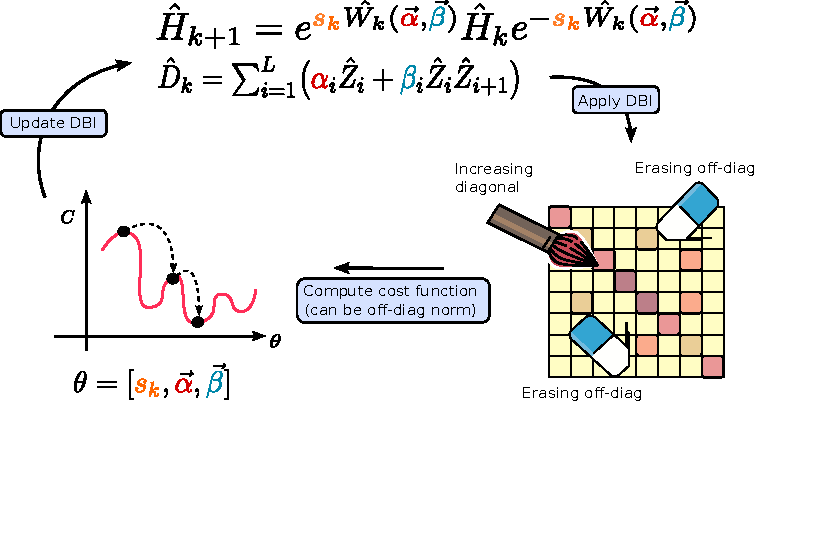
\includegraphics[width=1\textwidth]{figures/dbi_scheme_ink.pdf}
\end{figure}
\end{center}
\end{frame}

\begin{frame}{But how this can be a quantum algorithm? \hfill \href{https://arxiv.org/abs/2206.11772}{\textcolor{white}{\faBook\,\,arXiv:2206.11772}}}
The heart of the compilation of DBQAs is one of the \textbf{group commutator formulas} introduced
by Dawson and Nielsen in their \href{https://arxiv.org/abs/quant-ph/0505030}{Solovay-Kitaev algorithm}:
$$ \hat{V}^{\rm GC}(\hat{A}, \hat{B}) = e^{i\hat{A}} e^{i\hat{B}} e^{-i\hat{A}} e^{-i\hat{B}}, \qquad \qquad \hat{A}, \hat{B} \,\,\text{hermitian},$$
by means of which:
$$ e^{-[\hat{A}, \hat{B}]} = \hat{V}^{\rm GC}(\hat{A}, \hat{B}) + \hat{E}^{\rm GC}, $$
where 
$$  \hat{E}^{\rm GC} \leq \| [ \hat{A}, [\hat{A}, \hat{B}]] \| + \| [ \hat{B}, [\hat{B}, \hat{A}]] \|$$
in any unitarily invariant norm (e.g. Hilbert-Schmidt norm).

\begin{tcolorbox}[colback=red!15, title=How about DBI?]
$$ e^{- s [\hat{D}_0, \hat{H}_0]} = e^{i \sqrt{s_0}\hat{H}_0} 
e^{-i \sqrt{s_0}\hat{D}_0} e^{-i \sqrt{s_0}\hat{H}_0} e^{i \sqrt{s_0}\hat{D}_0} + O(s_0^{3/2}).$$
This is compilable into a sequence of local Hamiltonian evolutions.
\end{tcolorbox}
\faExclamationCircle\,\,Higher-order formulas can be implemented to reduce the approximation error.
\end{frame}

\begin{frame}{Warming start the new talk}
\begin{figure}
   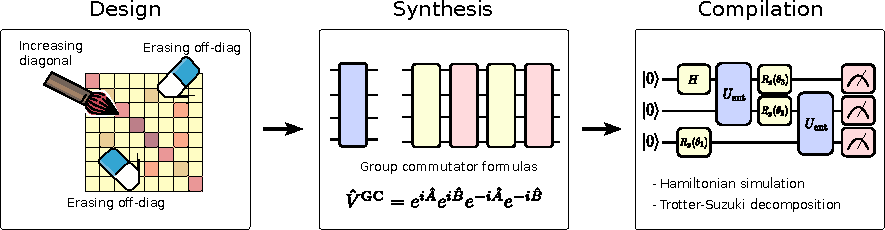
\includegraphics[width=1\textwidth]{figures/3_phases_dbqa.pdf}
\end{figure}
\end{frame}

\subtitle{\texttt{PART 2:} Interfacing DBQAs with other techniques}
\date{4 December 2024}

\begin{frame}{}
\maketitle
\end{frame}

\begin{frame}{A couple of references}
\begin{multicols}{2}
\begin{figure}
   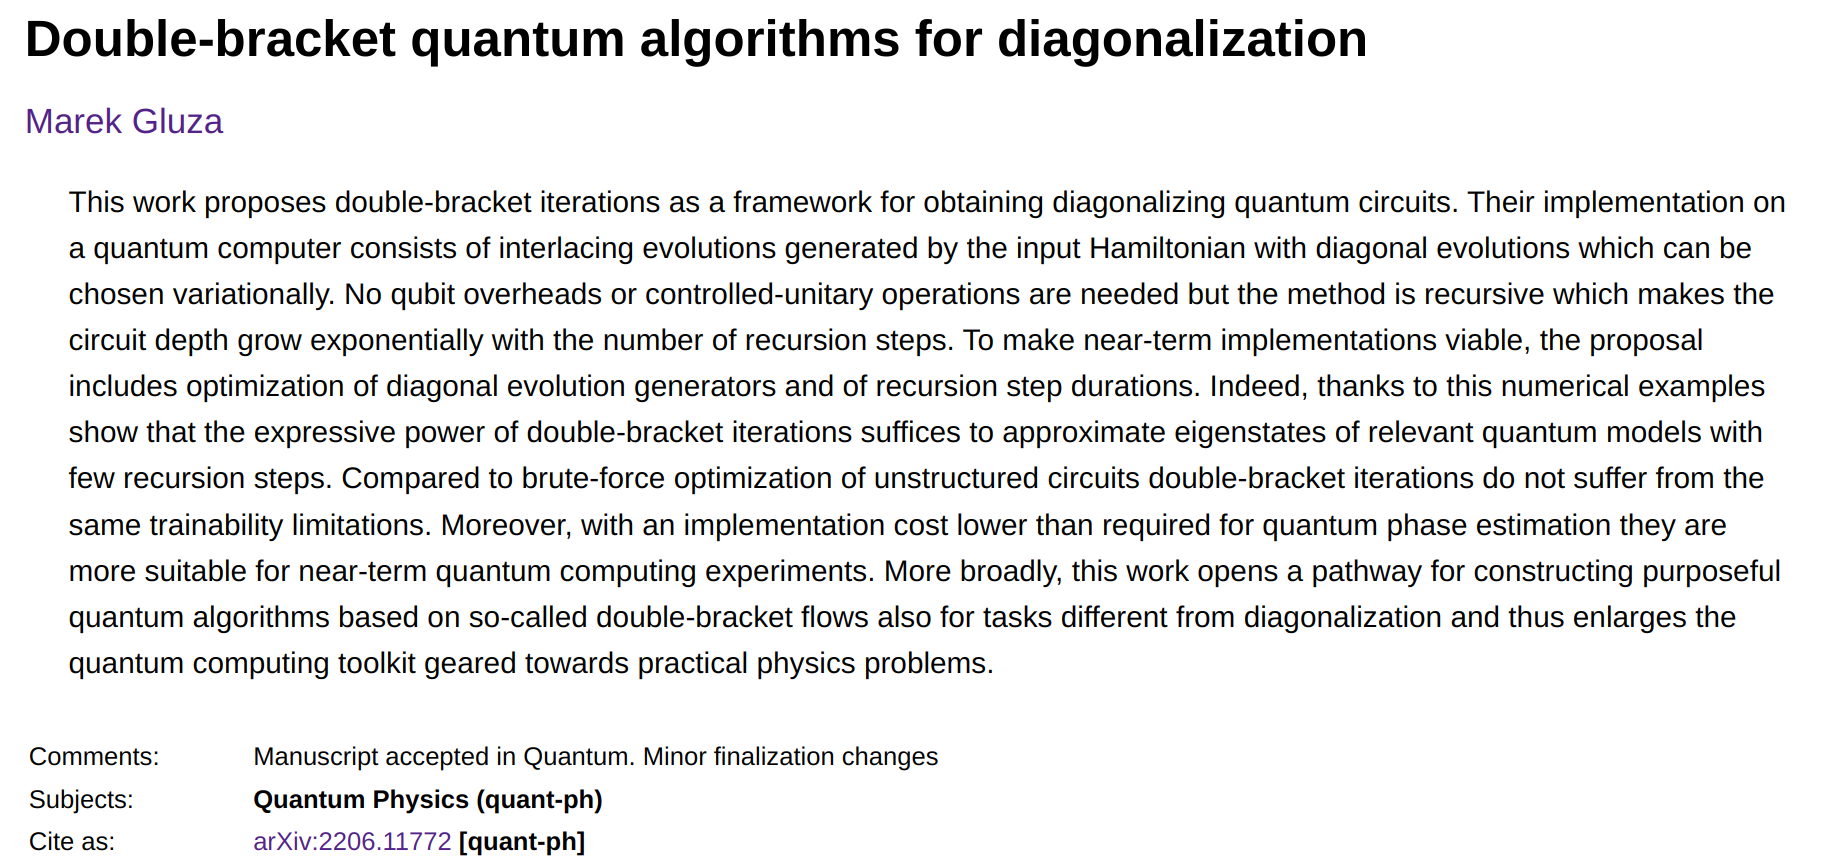
\includegraphics[width=0.5\textwidth]{figures/dbqa_paper.png}
\end{figure}
Check out this because:
\begin{itemize}[noitemsep]
\item[1.] Marek is a very nice and smart guy;
\item[2.] it contains math foundations of this talk; 
\end{itemize}
\begin{figure}
   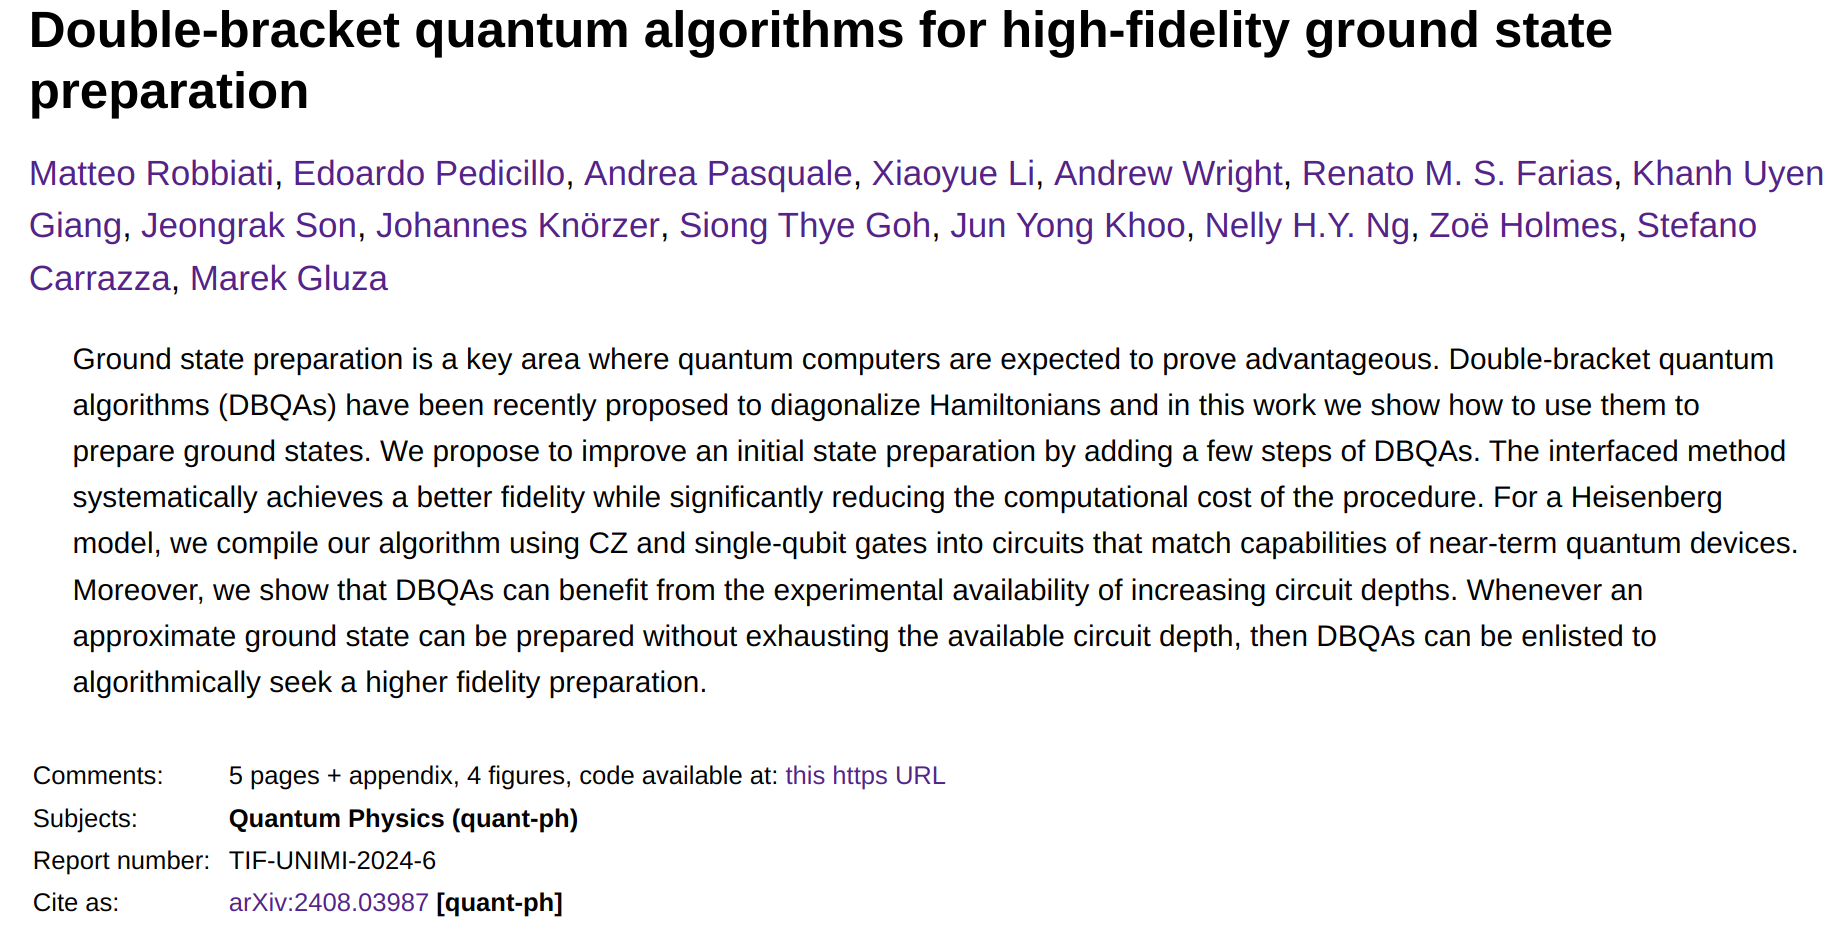
\includegraphics[width=0.5\textwidth]{figures/boostvqe_paper.png}
\end{figure}
And this because:
\begin{itemize}[noitemsep]
\item[1.] we will follow this paper for the numerical results;
\item[2.] there are some nice figures :) 
\end{itemize}
\end{multicols}
\end{frame}

\begin{frame}{Let's remember what a DBI is}
\begin{columns}[T,onlytextwidth]
    % First column: 40%
    \begin{column}{0.45\textwidth}
    \textbf{Ingredients}
        \begin{itemize}[noitemsep]
            \item[1.] Input Hamiltonian $\textcolor{mediumpersianblue}{\hat H_0}$ (here 1D XXZ);
            \item[2.] an anti-hermitian ($(i\hat{W})^{\dagger} = -i\hat{W}$) rotation generator $\textcolor{persianred}{\hat{W}_0} = [\hat{D}_0, \hat H_0]$;
            \item[3.] point 2. is used to build a unitary operation:
              $$ \hat{R}_0 \equiv e^{s \textcolor{persianred}{\hat{W}_0}}, $$
              with $s$ stepsize or flow duration;
            \item[4.] $\hat{R}_0$ applied to $\hat{H}_0$ as \textit{double-bracket rotation}:
               $$ \hat H_1 =  e^{s\textcolor{persianred}{\hat{W}_0}} \textcolor{mediumpersianblue}{\hat H_0} e^{- s \textcolor{persianred}{\hat{W}_0}}.$$
        \end{itemize}

    \end{column}

    % Second column: 60%
    \begin{column}{0.55\textwidth}
        \begin{figure}
           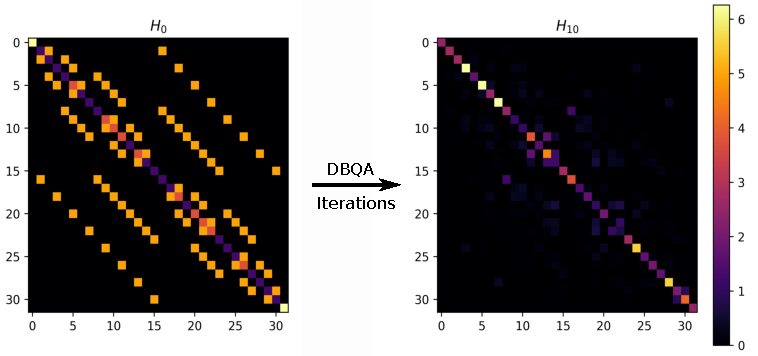
\includegraphics[width=0.95\textwidth]{figures/dbqa_10steps.pdf}
        \caption{Ten DBQA rotations to a 5 qubit 1D XXZ.}
        \end{figure}
    \end{column}
\end{columns}
\begin{tcolorbox}[colback=red!15, title=Nomenclature reason]
The presented framework satisfies a Heisenberg equation involving two, not one, brackets:
$$ \partial_s \hat{H}_0(s) = [ \hat{H}_0(s), [ \hat{H}_0(0), \hat{D}_0 ] ]. $$
\end{tcolorbox}
\end{frame}

\begin{frame}{How to make this work in practice?}
We left the last session with an approximation:
$$ e^{- s [\hat{D}, \hat{H}]} \approx e^{i \sqrt{s_k}\hat{H}_k} 
e^{i \sqrt{s_k}\hat{D}_k} e^{-i \sqrt{s_k}\hat{H}_k} e^{-i \sqrt{s_k}\hat{D}_k}.$$

Today, we will see how this is costly in practice, and propose the synergistic usage of 
more methods together.
\begin{figure}
   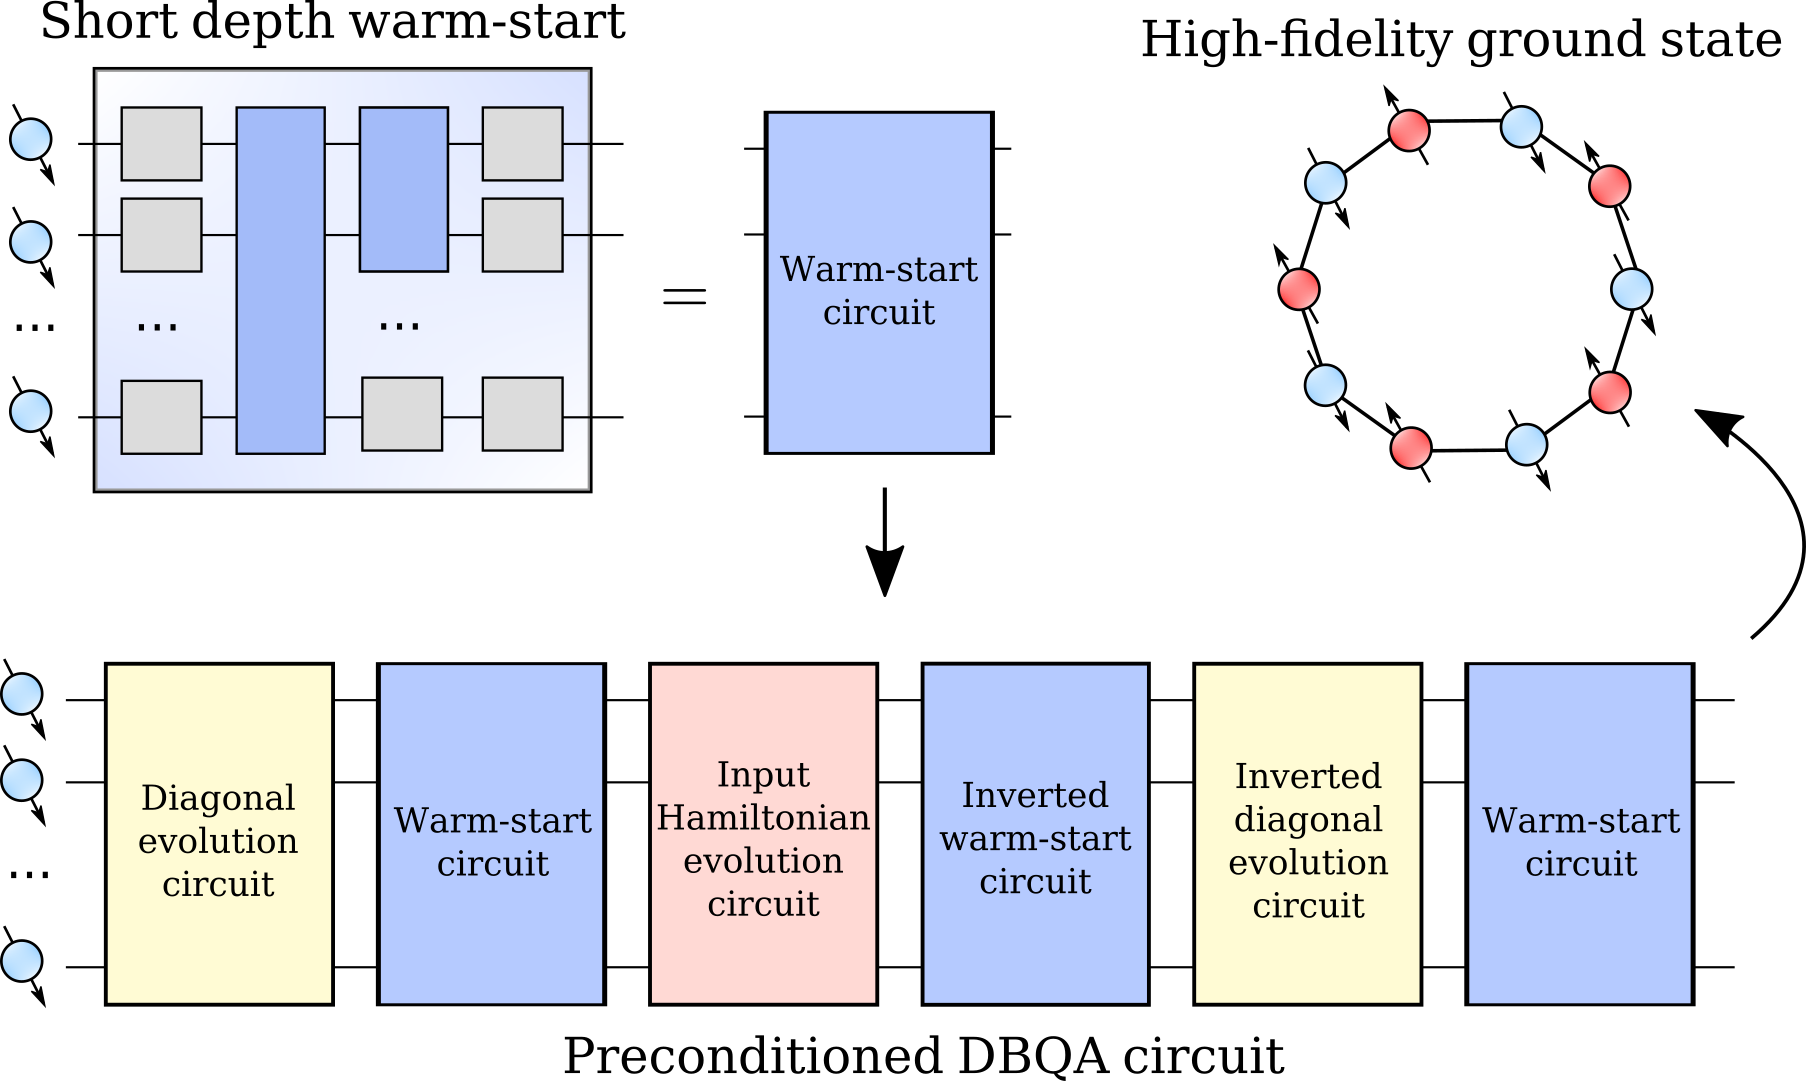
\includegraphics[width=0.6\textwidth]{figures/diagram.png}
\end{figure}
\end{frame}

\begin{frame}{Interfacing a warm start approximation with DBIs}
Let me apply a little modification to our input Hamiltonian:
$$ \hat{A}_0 = \hat{U}_{\theta}^{\dagger} \hat{H}_0 \hat{U}_{\theta}, $$
where $\hat{U}_{\theta}$ is a variational unitary operator introduced to approximate 
the ground state preparation (VQE here).
\begin{multicols}{2}
\vspace{1cm}
\texttt{  }

\textbf{VQE in a nutshell}
\begin{itemize}[noitemsep]
\item[1.] Define a good parametric circuit ansatz $\hat{U}_{\theta}$ (Hamming-weight preserving here);
\item[2.] we want the circuit to approximate the ground state of a target $\hat{H}_0$;
\item[3.] the cost function is the expval of $\hat{H}_0$ over the 
final state given by the circuit:
$$ C = \braket{0 | \hat{U}_{\theta}^{\dagger} \hat{H}_0  \hat{U}_{\theta} | 0}.$$
\end{itemize}
\begin{figure}
   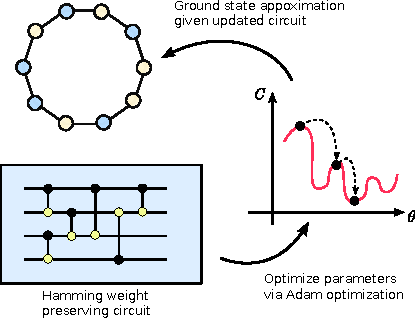
\includegraphics[width=0.45\textwidth]{figures/vqe_hw.pdf}
\end{figure}
\end{multicols}
\end{frame}

\begin{frame}{Interfacing a warm start approximation with DBIs}
Let me apply a little modification to our input Hamiltonian:
$$ \hat{A}_0 = \hat{U}_{\theta}^{\dagger} \hat{H}_0 \hat{U}_{\theta}. $$
One step of this group commutator iteration (GCI):
$$ \hat{A}_1 = \hat{V}_1^{\dagger} \hat{U}_{\theta}^{\dagger} \hat{H}_0 \hat{U}_{\theta} \hat{V}_1
\qquad \text{with} \qquad \hat{V}_1 =  e^{- i \sqrt{s_0}\hat{D}_0} \hat{U}_{\theta}^{\dagger} 
e^{- i \sqrt{s_0} \hat{H}_0}   \hat{U}_{\theta}  e^{i \sqrt{s_0}\hat{D}_0}. 
$$
Let me write here a (simplified in notation) full expression for the expval of $\hat{H}_0$:

$$ C = \braket{0| \textcolor{persianred}{e^{-D_0}} \textcolor{mediumpersianblue}{U^{\dagger}} 
e^{H_0} \textcolor{mediumpersianblue}{U}  \textcolor{persianred}{e^{D_0}} \textcolor{mediumpersianblue}{U^{\dagger}} 
H_0 \textcolor{mediumpersianblue}{U}  \textcolor{persianred}{e^{-D_0}} \textcolor{mediumpersianblue}{U^{\dagger}} e^{-H_0}  
\textcolor{mediumpersianblue}{U}  \textcolor{persianred}{e^{D_0}} |0} $$

\begin{tcolorbox}[colback=red!15, title=Reduced group commutator formula]
$$ \hat{V}^{(\rm RGC)}_k = e^{- i \sqrt{s_k}\hat{D}_k} e^{-i \sqrt{s_k}\hat{A}_k} e^{i \sqrt{s_k}\hat{D}_k} \qquad 
\text{since} \qquad \hat{A}_k =  e^{- i \sqrt{s_k}\hat{A}_k } \hat{A}_k e^{i \sqrt{s_k}\hat{A}_k }  $$ 
Cost reduction without any impact on the result calculation.
\end{tcolorbox}
\begin{picture}(0,0)
    \put(330,85){
        
\includegraphics[width=0.1\textwidth]{figures/feather_icon.png}
    }
\end{picture}
\end{frame}

\begin{frame}{Two steps}
In terms of state preparation (we want to compile it) one VQExDBQA step appears as:
$$ \textcolor{mediumpersianblue}{U}  \textcolor{persianred}{e^{-D_0}} \textcolor{mediumpersianblue}{U^{\dagger}} e^{-H_0}  
\textcolor{mediumpersianblue}{U}  \textcolor{persianred}{e^{D_0}} \ket{0}. $$
Adding one more step means applying $\hat{V}_2$ to the system:
\begin{align*}
   \hat V_2 
   =& e^{-ir_1 \D_1} \v_1^\dagger e^{-ir_1 \J_0} \v_1 e^{ir_1 \D_1}  \\
   =& 
   e^{-i(r_0 \D_0+r_1 \D_1)} \vqes^\dagger e^{ir_0 \h_0} \vqes e^{ir_0 \D_0} \vqes^\dagger e^{-ir_1 \h_0}\vqes
   e^{-ir_0 \D_0} \vqes^\dagger e^{-ir_0 \h_0} \vqes e^{i(r_0 \D_0+r_1 \D_1)}.
\end{align*}

\begin{tcolorbox}[colback=red!15, title=Compiling the hamiltonian evolutions]
The XXZ is decomposed into contributions involving two qubits per time $\hat{H}_0 = \sum_{a=1}^L \hat{H}^{(a)}$ such that
$\hat{H}^{(a)} = \hat{X}_a \hat{X}_{a+1} + \hat{Y}_a \hat{Y}_{a+1} + \hat{Z}_a \hat{Z}_{a+1}$ and then a Trotter-Suzuki decomposition
is implemented:
\begin{align*}
	e^{-it \h_0} = \left( \prod_{a=1}^L e^{-i\frac{t}{M}\h^{(a)}}\right)^M+O(M^{-1}).
\end{align*}
\end{tcolorbox}
\begin{picture}(0,0)
    \put(340,125){
        
\includegraphics[width=0.15\textwidth]{figures/explosion_icon.png}
    }
\end{picture}
\end{frame}

\begin{frame}{Compiling}
\begin{multicols}{2}
\textbf{Any unitary can be compiled into proper set of gates}
\begin{itemize}[noitemsep]
\item[1.] Euler decomposition for 1-qubit gates;
\item[2.] KAK decomposition for 2-qubit gates;
\item[3.] Shannon decomposition for n-qubit gates.
\end{itemize}
\begin{figure}
   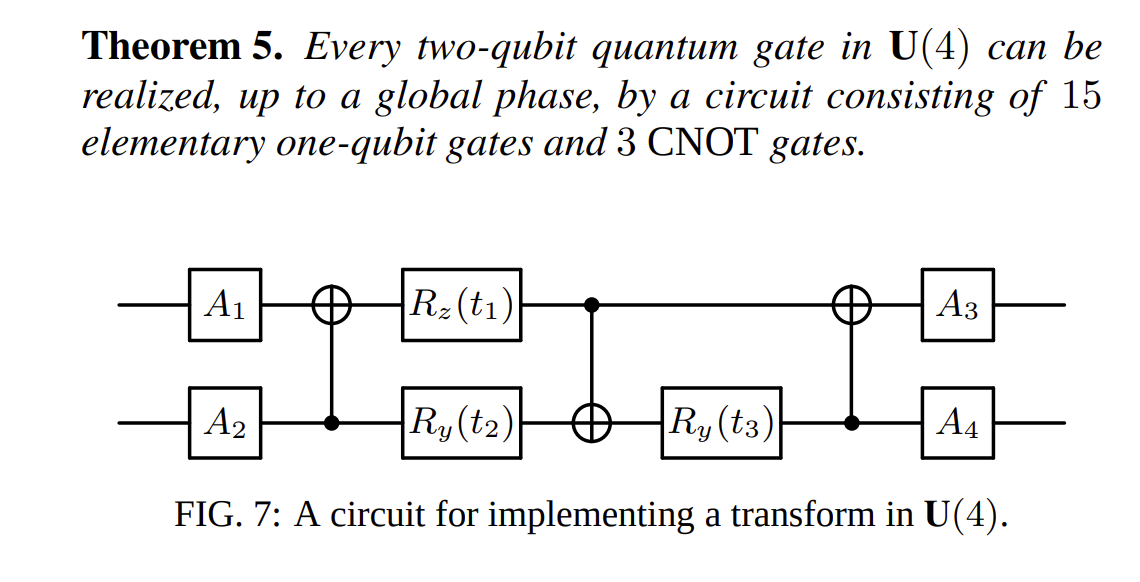
\includegraphics[width=0.5\textwidth]{figures/2q_compilation.png}
\end{figure}
\end{multicols}
Trotter-Suzuki approximation, combined with compilation, means a quite intense 
number of required gates.
\begin{tcolorbox}[colback=red!15, title=\faLightbulbO\,\,\,Interface with a warm start a a couple of DBI steps]
If we are able to setup a short-depth first approximation, then we can boost the preparation with DBI.
\end{tcolorbox}
\begin{picture}(0,0)
    \put(30,75){
        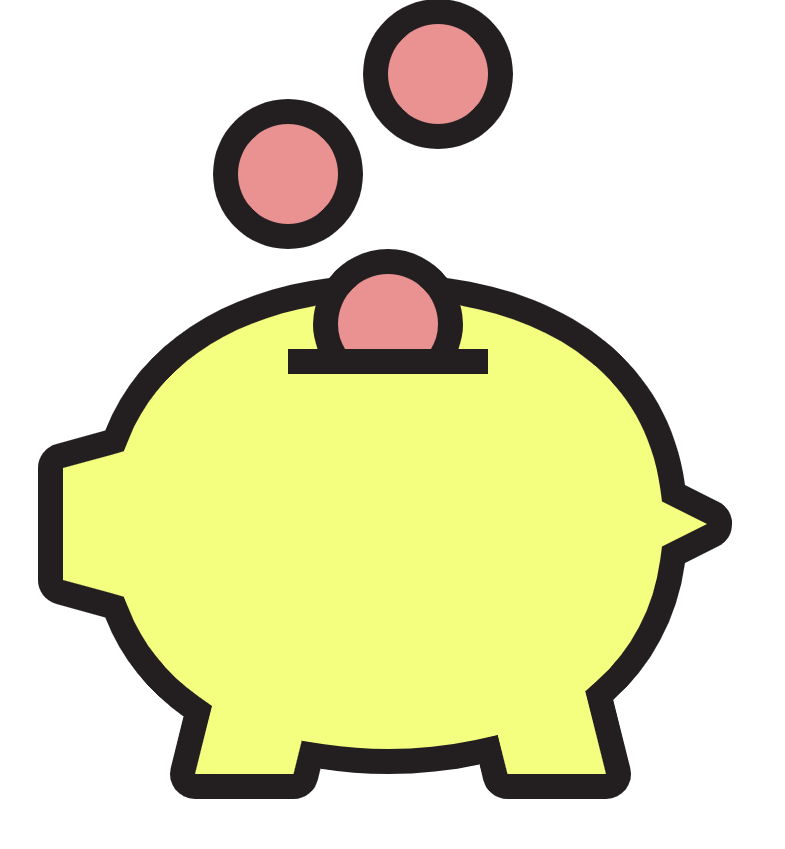
\includegraphics[width=0.1\textwidth]{figures/save_coin.png}
    }
\end{picture}
\end{frame}

\begin{frame}{Boosting 1D XXZ ground state preparation}
\begin{figure}
   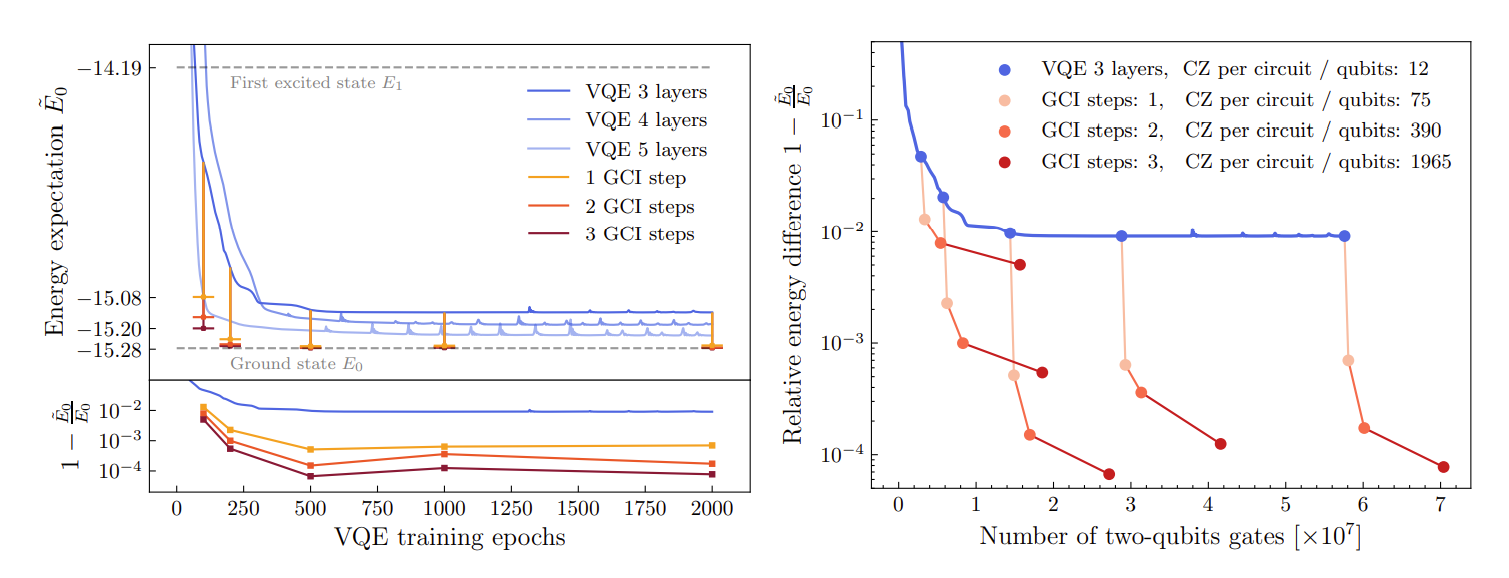
\includegraphics[width=1\textwidth]{figures/results_hw.png}
\end{figure}
\begin{tcolorbox}[colback=red!15, title=\faLightbulbO\,\,\,Two qubit gates count]
Number of CZ executed considering \textit{i)} VQE training, 
\textit{ii)} hyper-optimization of the unfolded GCI's parameters.
\end{tcolorbox}
\end{frame}

\begin{frame}{Optimization reminder \hfill \href{https://arxiv.org/abs/2408.07431}{\textcolor{white}{\faBook\,\,arXiv:2408.07431}}}
\begin{center}
\begin{figure}
   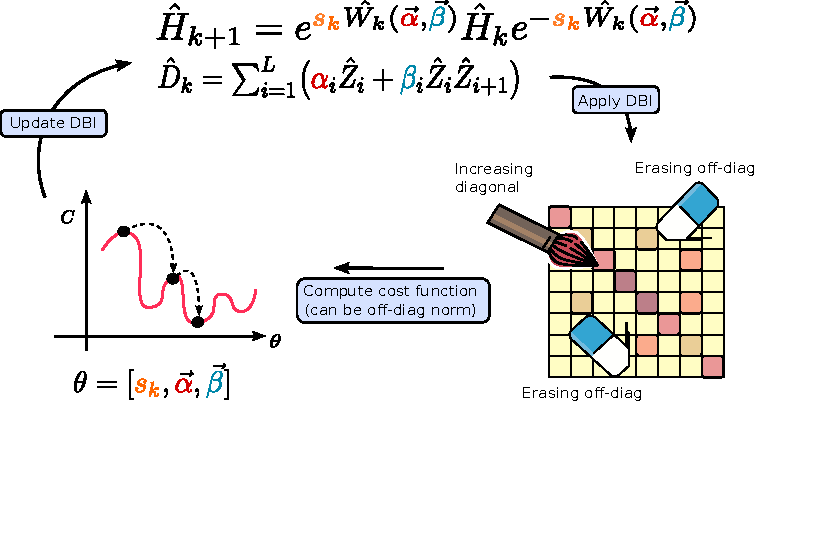
\includegraphics[width=1\textwidth]{figures/dbi_scheme_ink.pdf}
\end{figure}
\end{center}
\begin{picture}(0,0)
    \put(100,175){
        
\includegraphics[width=0.1\textwidth]{figures/cma_icon.png}
    }
\end{picture}
\end{frame}

\begin{frame}{Boosting 1D XXZ ground state preparation}
\begin{figure}
   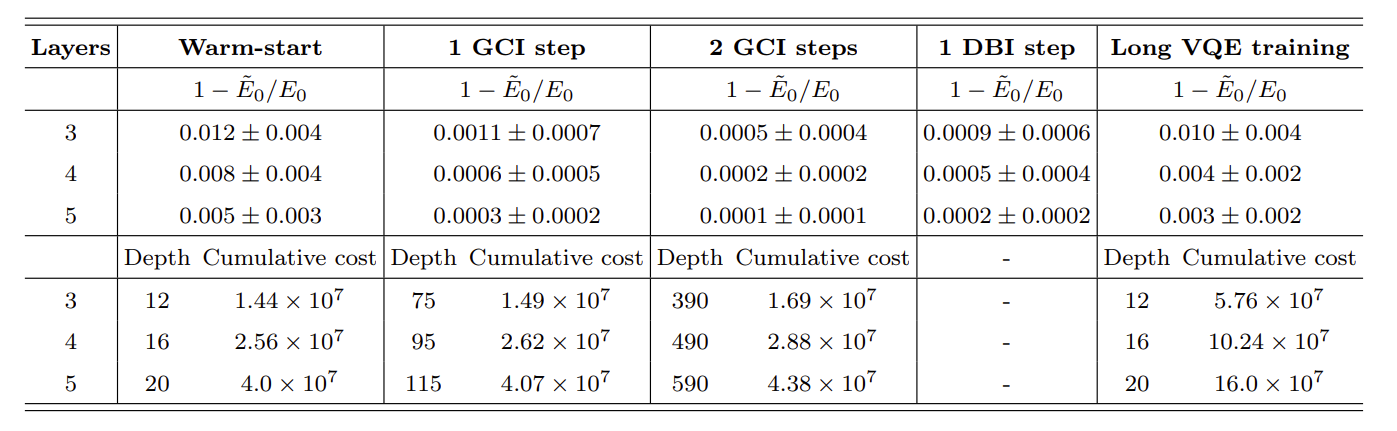
\includegraphics[width=0.8\textwidth]{figures/table_hw.png}
\end{figure}
\begin{flushleft}
   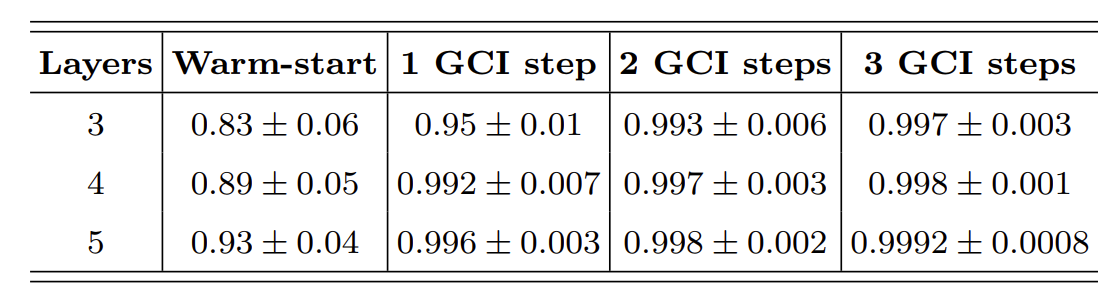
\includegraphics[width=0.5\textwidth]{figures/fidelity_hw.png}
\end{flushleft}
\begin{picture}(0,0)
    \put(220,-15){
        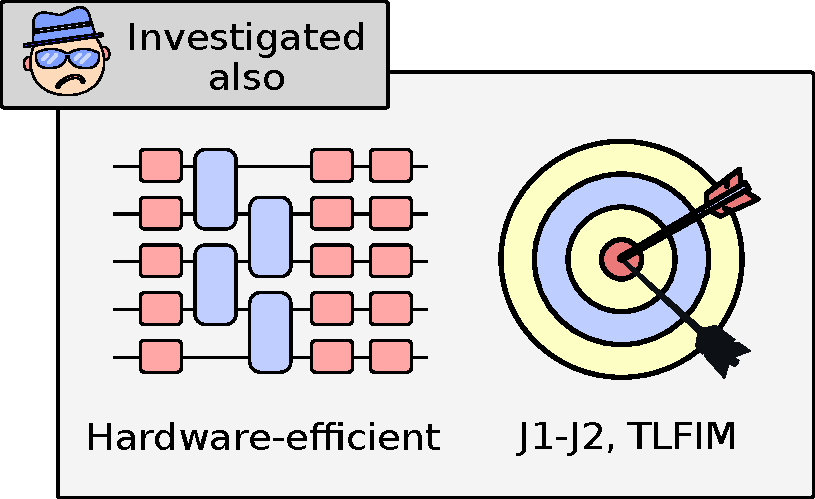
\includegraphics[width=0.37\textwidth]{figures/investigated_also.pdf}
    }
\end{picture}
\end{frame}

\end{document}




